\begin{figure}[htbp]
    \centering
    \begin{minipage}[ht]{0.48\hsize}\centering
        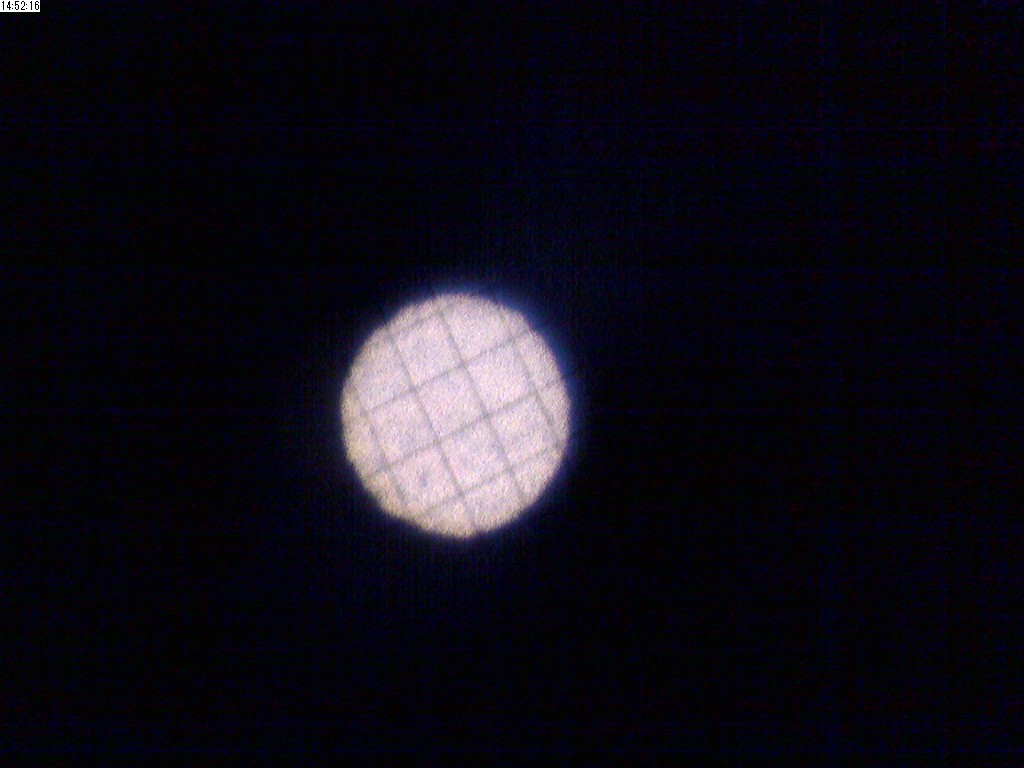
\includegraphics[width=\linewidth]{src/figures/result/circle_slit.jpg}
        \subcaption{円スリット}\label{subfig:circle_slit}
    \end{minipage}
    \begin{minipage}[ht]{0.48\hsize}\centering
        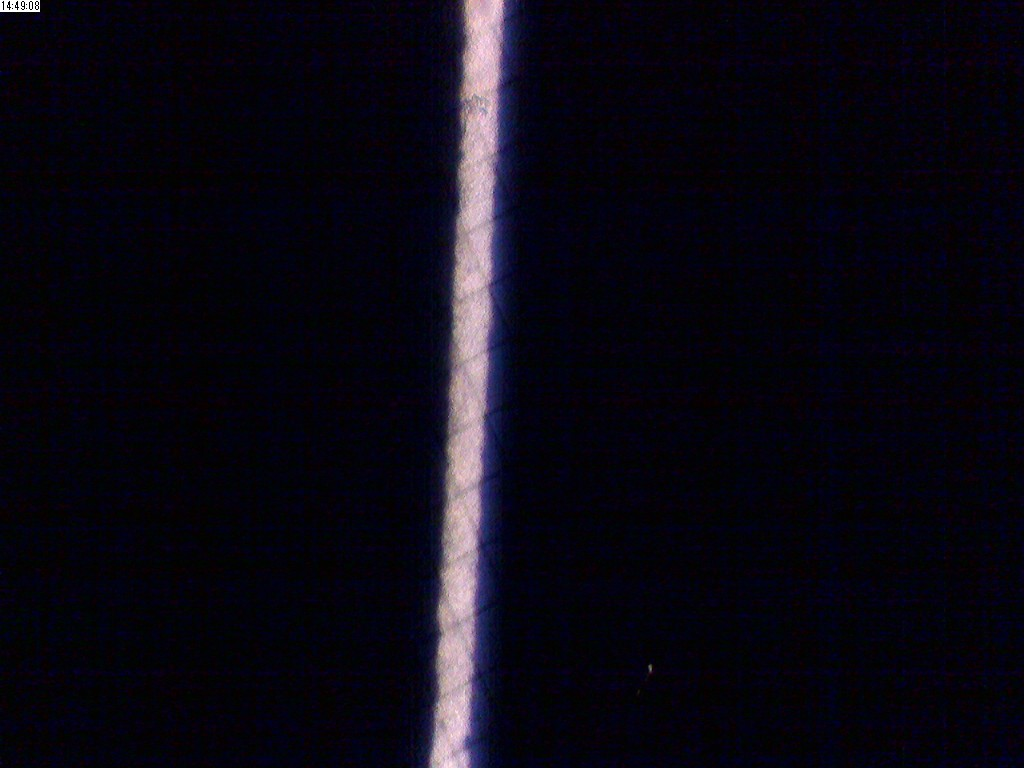
\includegraphics[width=\linewidth]{src/figures/result/ss1_slit.jpg}
        \subcaption{単スリット1}\label{subfig:ss1_slit}
    \end{minipage}
    \begin{minipage}[ht]{0.48\hsize}\centering
        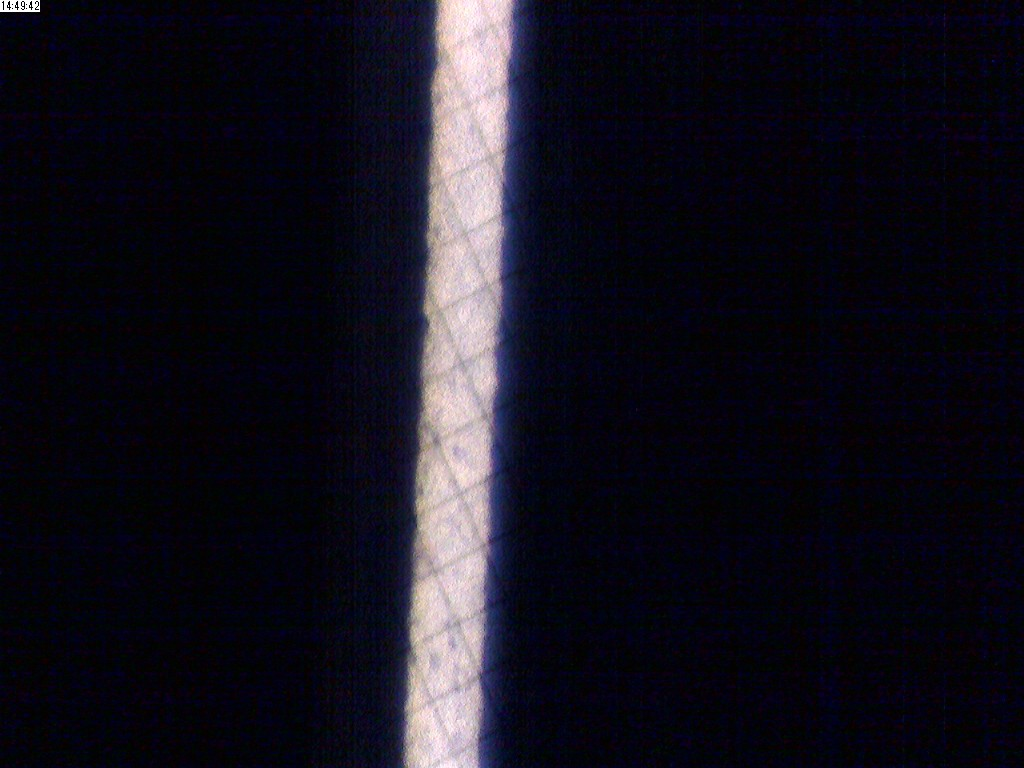
\includegraphics[width=\linewidth]{src/figures/result/ss2_slit.jpg}
        \subcaption{単スリット2}\label{subfig:ss2_slit}
    \end{minipage}
    \begin{minipage}[ht]{0.48\hsize}\centering
        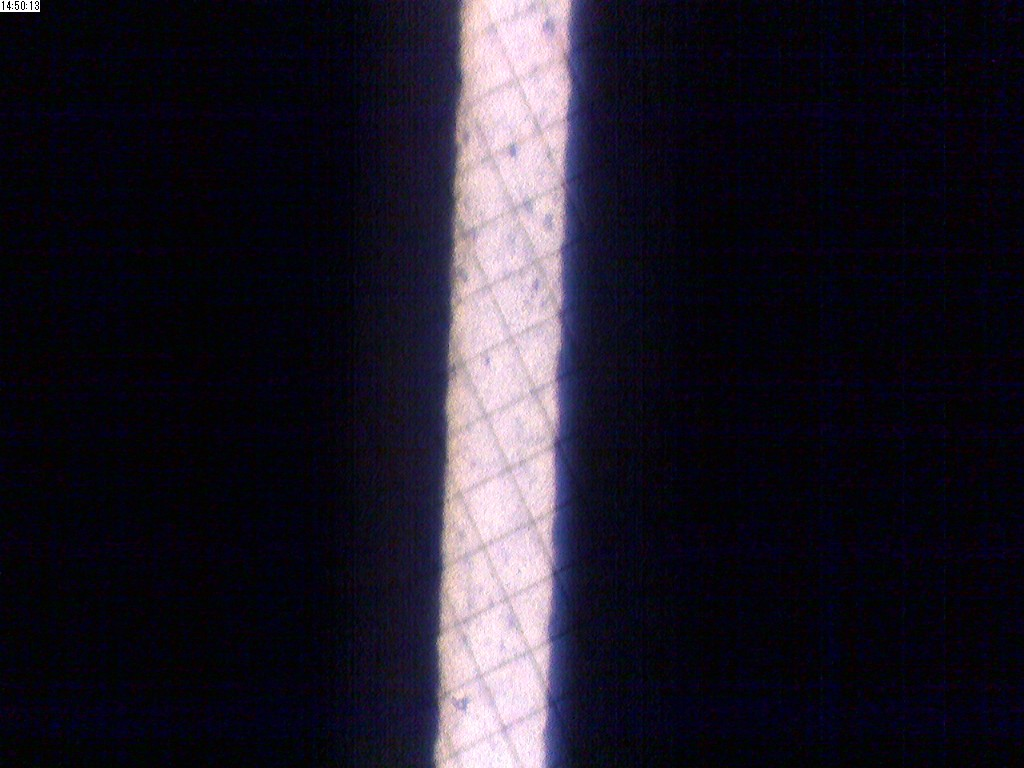
\includegraphics[width=\linewidth]{src/figures/result/ss3_slit.jpg}
        \subcaption{単スリット3}\label{subfig:ss3_slit}
    \end{minipage}
    \begin{minipage}[ht]{0.48\hsize}\centering
        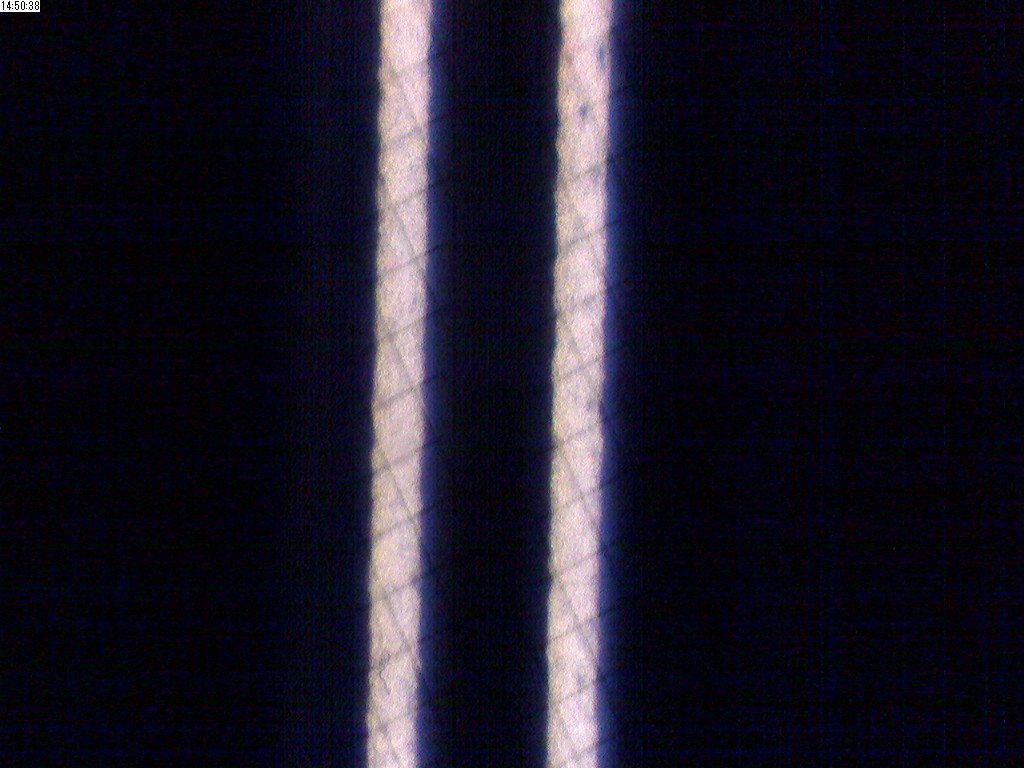
\includegraphics[width=\linewidth]{src/figures/result/ds1_slit.jpg}
        \subcaption{ダブルスリット1}\label{subfig:ds1_slit}
    \end{minipage}
    \begin{minipage}[ht]{0.48\hsize}\centering
        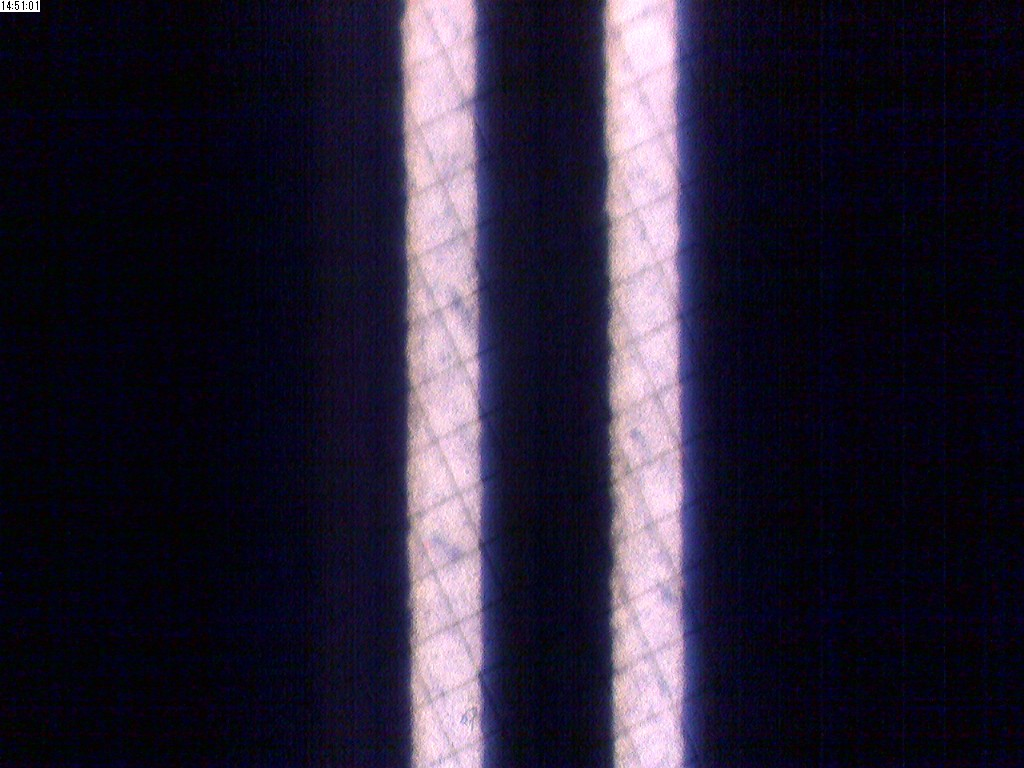
\includegraphics[width=\linewidth]{src/figures/result/ds2_slit.jpg}
        \subcaption{ダブルスリット2}\label{subfig:ds2_slit}
    \end{minipage}
\end{figure}
\begin{figure}[htbp]
    \centering
    \addtocounter{figure}{-1}
    \begin{subfigure}{0.48\hsize}\centering
        \addtocounter{subfigure}{6}
        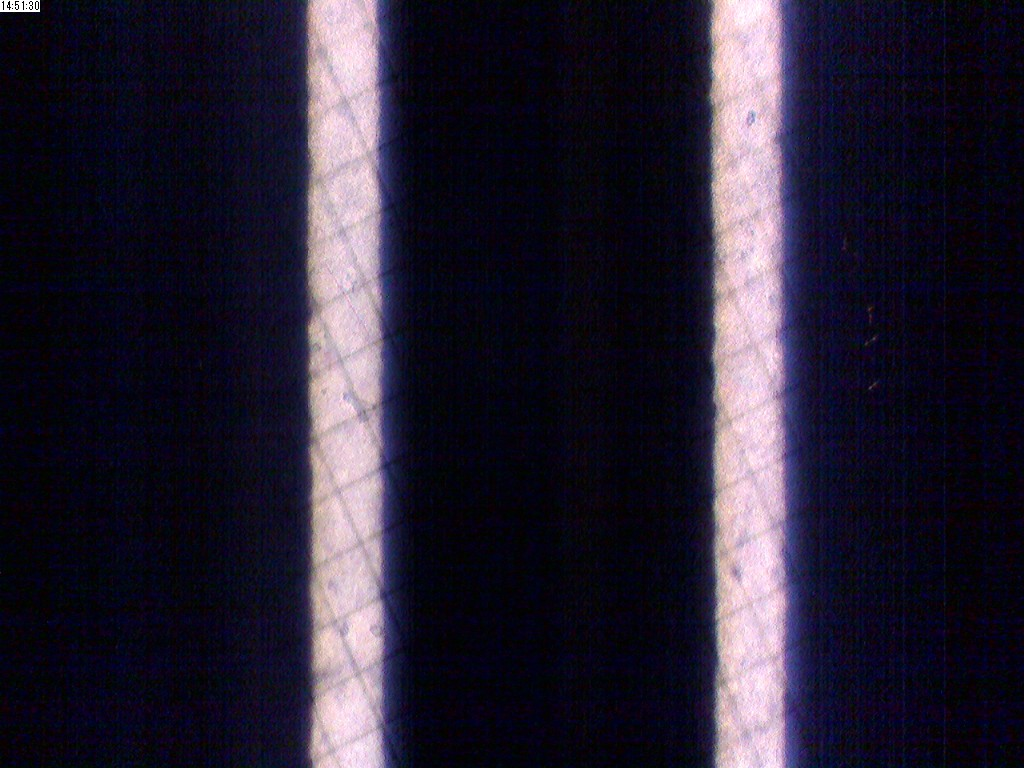
\includegraphics[width=\linewidth]{src/figures/result/ds3_slit.jpg}
        \subcaption{ダブルスリット3}\label{subfig:ds3_slit}
    \end{subfigure}
    % \begin{subfigure}{0.48\hsize}
    %     \includegraphics[width=\linewidth]{src/figures/result/square.jpg}
    %     \subcaption{正方形}\label{subfig:square_slit}
    % \end{subfigure}
    % \begin{minipage}[ht]{0.48\hsize}\centering
    %     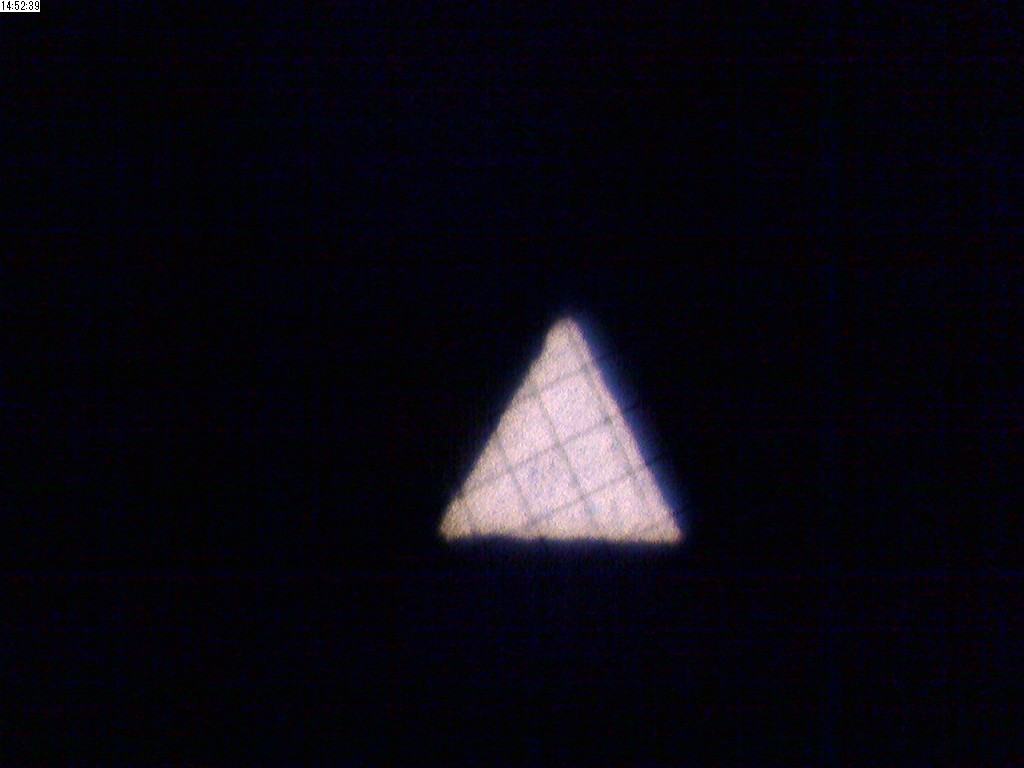
\includegraphics[width=\linewidth]{src/figures/result/triangle_slit.jpg}
    %     \subcaption{三角形スリット}\label{subfig:triangle_slit}
    % \end{minipage}
    \begin{subfigure}{0.48\hsize}\centering
        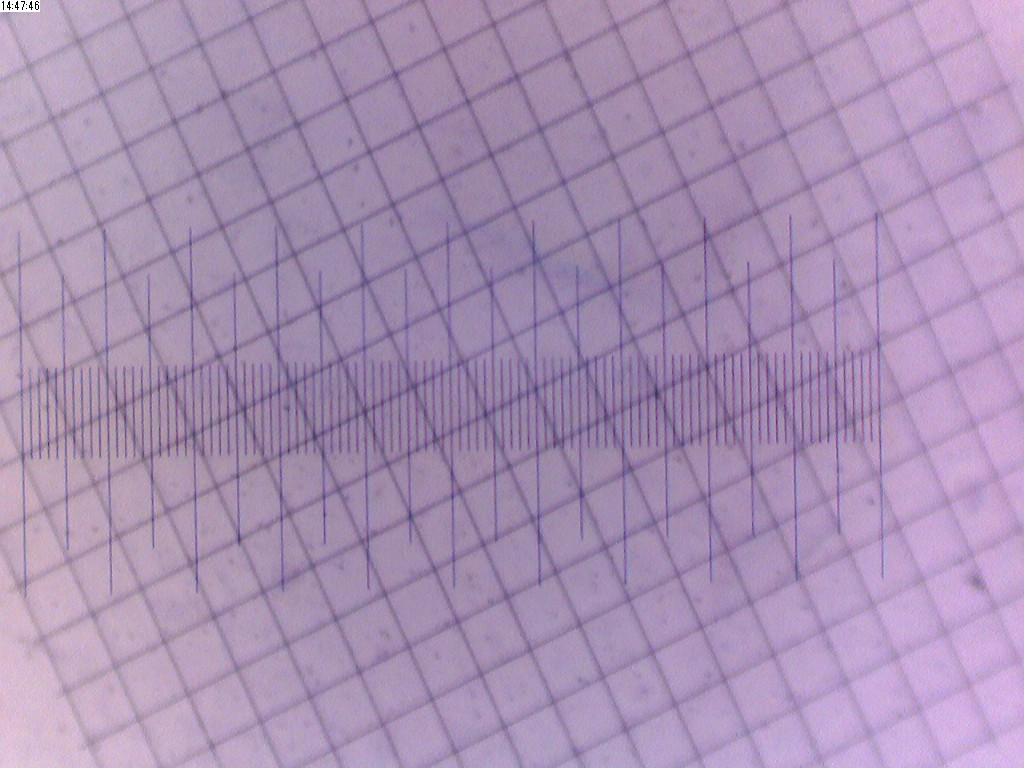
\includegraphics[width=\linewidth]{src/figures/result/meaure_slit.jpg}
        \subcaption{定規}\label{subfig:measure}
    \end{subfigure}
    \caption{スリットの画像}\label{fig:slit_image}
\end{figure}
